\subsection{Example \#3: time series with anomaly}
\label{S:ExampleDispAnomaly}


\subsubsection{Data description}
This example uses a synthetic time series that mimics displacement data measured on a bridge. 
The Figure~\ref{fig:DataSummaryRaw3}a shows that data points exist between May 2008 and April 2012.
The timestep is non-uniform; it varies from 1 hour to 10 days (see Figure~\ref{fig:DataSummaryRaw3}b). 
The most frequent (i.e referent) time step is 12 hour (see Section~\ref{SS:NonUniform}).
There is no missing data on the displacement time series.
The baseline switches between a trend stationary to acceleration stationary dynamics during a specific time window to mimic a fictitious anomaly.
The anomaly time window has a length of 26 days, starting on June 25, 2010.
The displacement also exhibits a yearly periodic and autoregressive patterns.

\begin{figure*}[h!]
\centering
\begin{subfigure}{\linewidth}
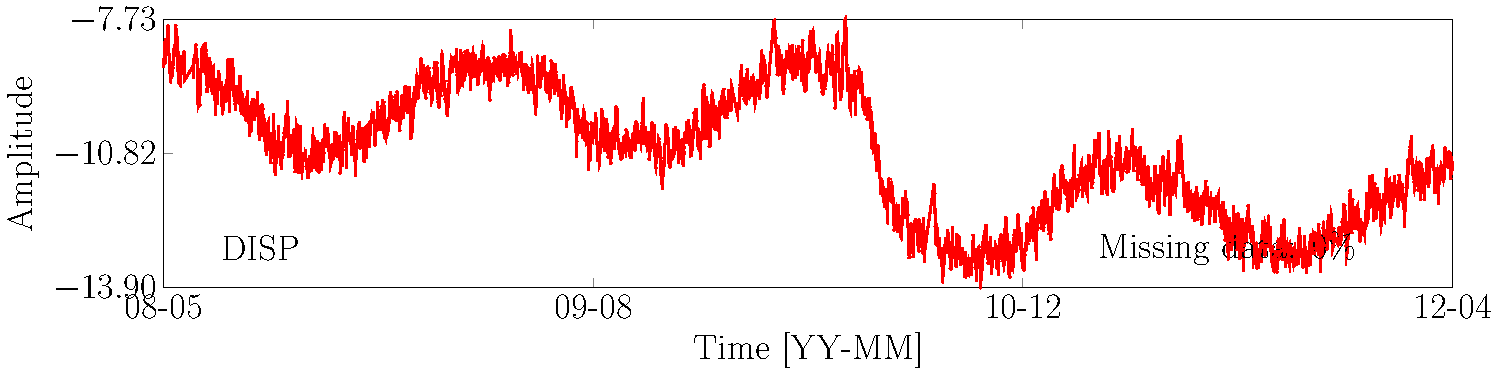
\includegraphics[width=0.9\linewidth]{./docfigs/Example_DISPSIM_ANOMALY/raw/ALL_AMPLITUDES.pdf} 
\caption{Amplitude}
\end{subfigure}
\begin{subfigure}{\linewidth}
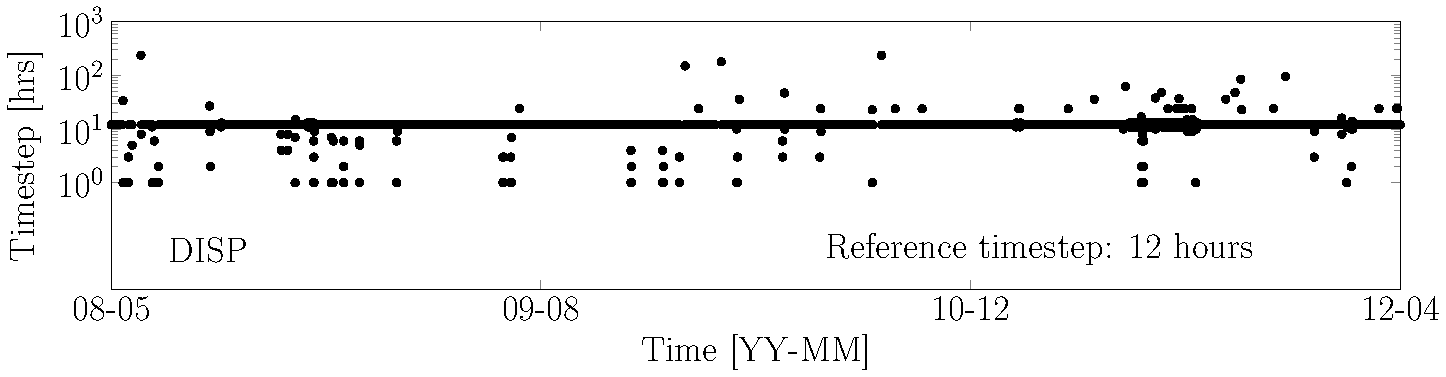
\includegraphics[width=0.9\linewidth]{./docfigs/Example_DISPSIM_ANOMALY/raw/ALL_TIMESTEPS.pdf}
\caption{Timestep}
\end{subfigure}
\begin{subfigure}{\linewidth}
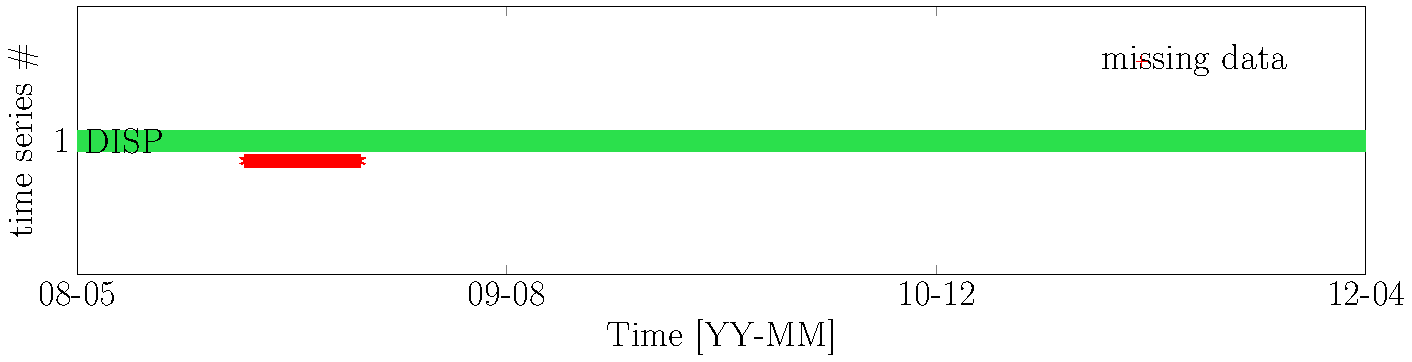
\includegraphics[width=0.9\linewidth]{./docfigs/Example_DISPSIM_ANOMALY/raw/AVAILABILITY.pdf}
\caption{Availability}
\end{subfigure}
\caption{Data used in example \#3}.
\label{fig:DataSummaryRaw3}
\end{figure*}



\subsubsection{Model description}
\label{SS:ModelConstructionExample3}
The model includes two model classes, and the block components are 
\begin{gather*}
\mathbf{x}^{1}=[x^{\mathtt{L}}, x^{\mathtt{LT}}, x^{\mathtt{LAc}}, x^{\mathtt{P1}\text{,yearly}} , x^{\mathtt{P2}\text{,yearly}}, x^{\mathtt{AR}}]
 \end{gather*}
for the model class \#1, and
\begin{gather*}
\mathbf{x}^{2}=[x^{\mathtt{L}}, x^{\mathtt{LT}}, x^{\mathtt{LA}}, x^{\mathtt{P1}\text{,yearly}} , x^{\mathtt{P2}\text{,yearly}}, x^{\mathtt{AR}}]
 \end{gather*}
for the model class \#2.
The associated model parameters are
\begin{gather*}
\bm\theta=[sigma_{w}^{\mathtt{TcA},1}, p^{\mathtt{P}, \text{yearly}}, \sigma_{w}^{\mathtt{P}, \text{yearly}}, \phi^{\mathtt{AR}}, \sigma_{w}^{\mathtt{AR}}, \\
 \sigma_{w}^{\mathtt{LA},2}, \sigma_{w}^{\mathtt{TcA}, 12}, \sigma_{w}^{\mathtt{LA}, 21}, \sigma^{1}_{v}, \sigma^{2}_{v}, Z^{11},   Z^{22}] \text{.}
 \end{gather*}
The optimized model parameters values computed using the Newton-Raphson algorithm (see~\ref{SS:THModelParameterEstimation}) are
\begin{gather*}
\bm\theta^{\text{*}}=[0, 365.24, 0, 0.75, 0.213, \\
0.001, 8.1224\times10^{-6}, 1.5018\times10^{-5}, 0.10671, 0.10671, 0.99997, 0.99957].
\end{gather*}
The optimized initial hidden states mean, covariance  and model probability values for model class \#1 are 
\begin{align*}
 \bm \mu^{1,\text{*}}_{0} & = [	-9.43 ,	-0.0109	, -5.03\times 10^{-9}	, 1.08  ,	-0.00634	, -0.548    ]^{\intercal}, \text{and} \\
\bm\Sigma^{1,\text{*}}_{0}  & = \text{diag}[	0.139 ,	0.000877,	2.26  	,0.00224	,0.00105,	0.32     ],  \text{and} \\
 \pi_{0}^{1,\text{*}} & = 0.997.
\end{align*}
The optimized initial hidden states mean, covariance  and model probability values for model class \#2 are 
\begin{align*}
 \bm \mu^{2,\text{*}}_{0} & = [	-9.53 ,	0.102 ,	-0.0599	,  1.08  ,	-0.00636, 	-0.482     ]^{\intercal}, \text{and} \\
 \bm\Sigma^{2,\text{*}}_{0}  & = \text{diag}[	0.674 	,0.418 ,	0.803 ,	0.00224,	0.00105	, 0.759    ], \text{and} \\
 \pi_{0}^{2,\text{*}} & = 0.00279.
\end{align*}
The hidden states computed using the estimated model parameters and initial hidden states are presented in Figure~\ref{fig:DISPSIMANOMALYOptimizedOptimizedExample3}.

\begin{figure*}[h!]
\centering
\begin{subfigure}{\linewidth}
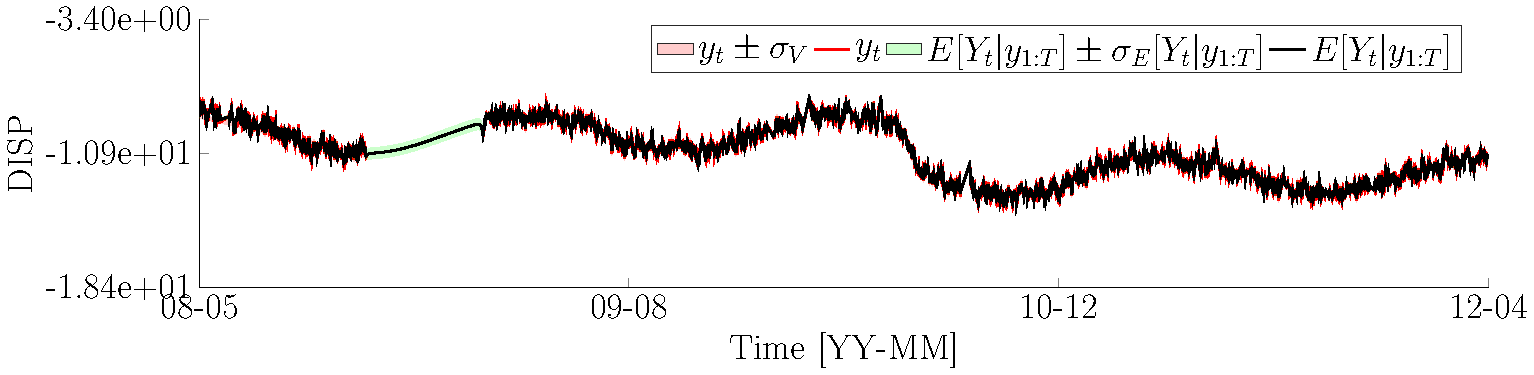
\includegraphics[width=0.9\linewidth]{./docfigs/Example_DISPSIM_ANOMALY/optim_param_optim_initialhiddenstate/DISP_ObservedPredicted.pdf}
\caption{Observed and estimated displacement data}
\end{subfigure}
\begin{subfigure}{\linewidth}
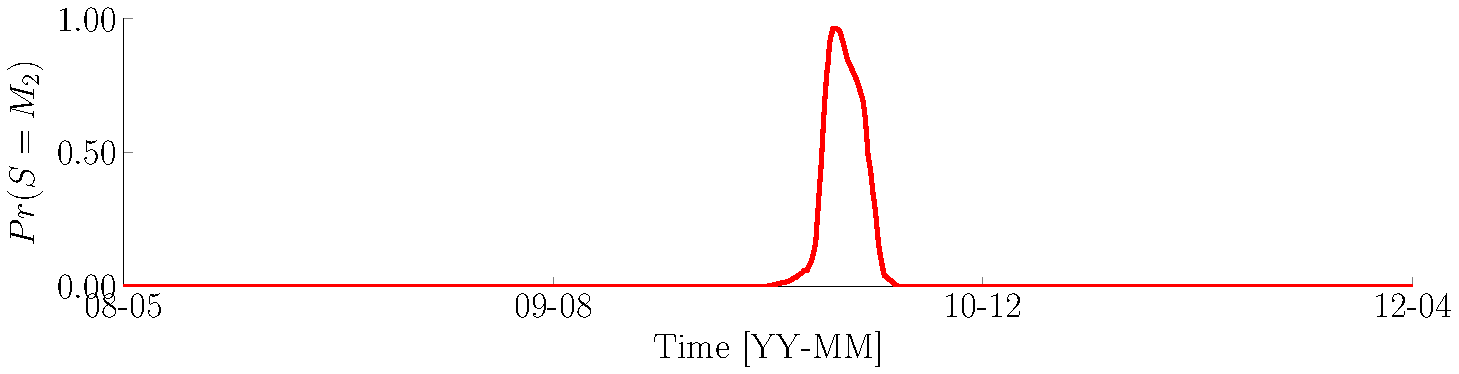
\includegraphics[width=0.9\linewidth]{./docfigs/Example_DISPSIM_ANOMALY/optim_param_optim_initialhiddenstate/ModelProbability.pdf} 
\caption{Estimated probability of anomaly (probability of model class 2)}
\end{subfigure}
\begin{subfigure}{\linewidth}
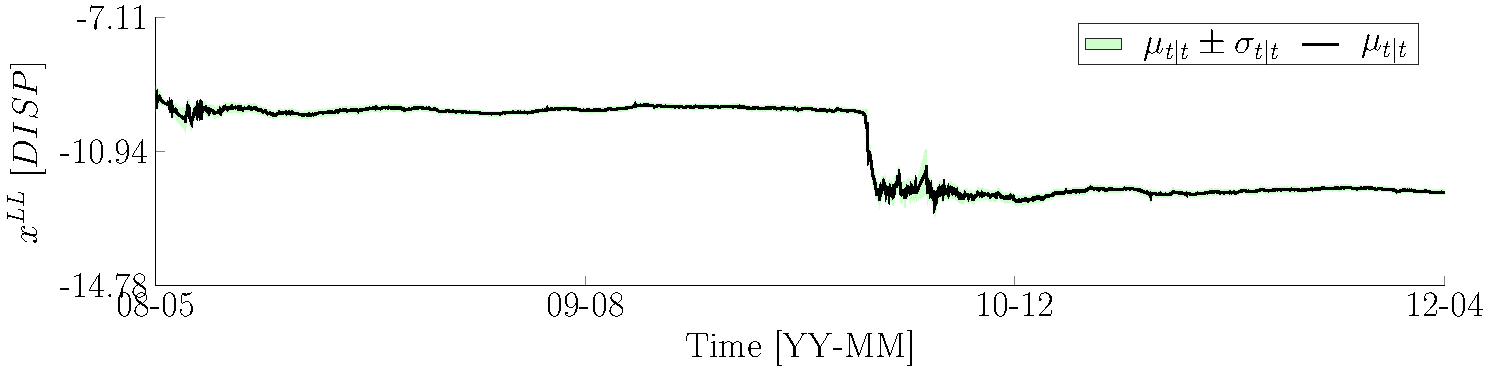
\includegraphics[width=0.9\linewidth]{./docfigs/Example_DISPSIM_ANOMALY/optim_param_optim_initialhiddenstate/DISP_LL_1.pdf} 
\caption{Estimated displacement level component}
\end{subfigure}
\begin{subfigure}{\linewidth}
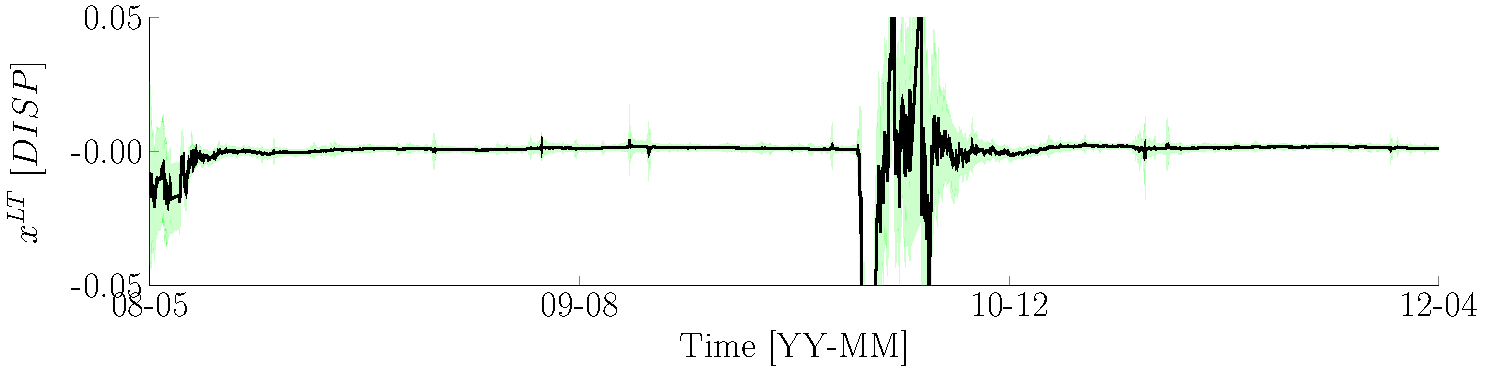
\includegraphics[width=0.9\linewidth]{./docfigs/Example_DISPSIM_ANOMALY/optim_param_optim_initialhiddenstate/DISP_LT_2.pdf}
\caption{Estimated displacement local trend component.}
\end{subfigure}
\begin{subfigure}{\linewidth}
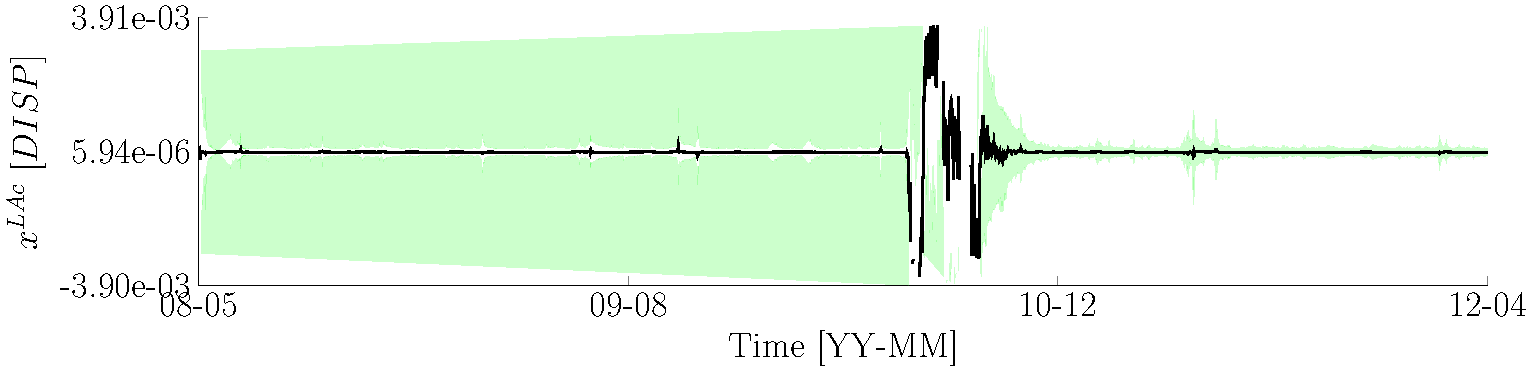
\includegraphics[width=0.9\linewidth]{./docfigs/Example_DISPSIM_ANOMALY/optim_param_optim_initialhiddenstate/DISP_LAc_3.pdf}
\caption{Estimated displacement local acceleration component.}
\end{subfigure}
\end{figure*}
\begin{figure*}[h!]
\ContinuedFloat
\begin{subfigure}{\linewidth}
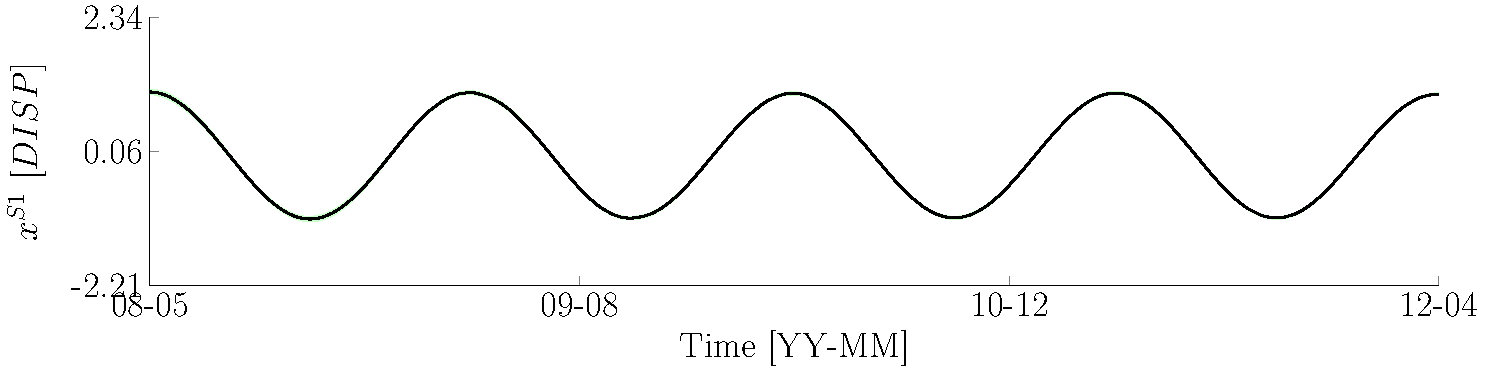
\includegraphics[width=0.9\linewidth]{./docfigs/Example_DISPSIM_ANOMALY/optim_param_optim_initialhiddenstate/DISP_S1_4.pdf}
\caption{Estimated displacement yearly periodic component (first hidden state)}
\end{subfigure}
\begin{subfigure}{\linewidth}
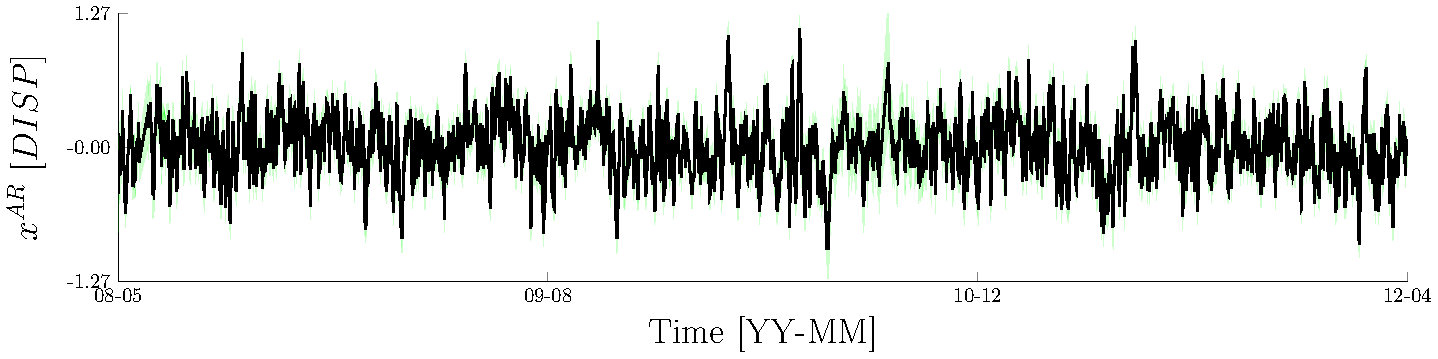
\includegraphics[width=0.9\linewidth]{./docfigs/Example_DISPSIM_ANOMALY/optim_param_optim_initialhiddenstate/DISP_AR_6.pdf} 
\caption{Estimated displacement autoregressive component}
\end{subfigure}
\caption{Estimated results using OpenBDLM optimized model parameters and optimized initial hidden states. The hidden states are estimated from the data presented in Figure~\ref{fig:DataSummaryRaw3}a. The solid line and shaded area represent the mean and standard deviation of the estimated hidden states, respectively.}
\label{fig:DISPSIMANOMALYOptimizedOptimizedExample3}
\end{figure*}



\subsubsection{Run the example from pre-existing configuration file}
\label{SS:LoadConfigFileEx3}

There is a configuration file CFG\_Example\_DISP\_ANOMALY\_optim.m which is located in the ``config\_files'' folder of the OpenBDLM package.
CFG\_Example\_DISP\_ANOMALY\_optim.m contains the optimized model parameters and optimized initial hidden states values.
There is also a data file DATA\_Example\_DISP\_ANOMALY\_optim.mat that is located in the ``data/mat'' subfolder.
Therefore, it is possible to run the example \#3 by following the following steps from the \MATLAB{} command line:
\begin{enumerate}
\item Start OpenBDLM. Type \colorbox{light-gray}{\lstinline[basicstyle = \mlttfamily \small, backgroundcolor = \color{light-gray}]!OpenBDLM_main('CFG_Example_DISP_ANOMALY_optim.m');!}.
\item Access hidden states estimation menu. Type \colorbox{light-gray}{\lstinline[basicstyle = \mlttfamily \small, backgroundcolor = \color{light-gray}]!3!}.
\item Run the Kalman filter to estimate the hidden states. Type \colorbox{light-gray}{\lstinline[basicstyle = \mlttfamily \small, backgroundcolor = \color{light-gray}]!1!}.
\item Save and quit. Type \colorbox{light-gray}{\lstinline[basicstyle = \mlttfamily \small, backgroundcolor = \color{light-gray}]!Q!}.
\end{enumerate}


\subsubsection{Run the example from command line interaction}

The analysis of a new dataset usually requires to start from scratch.
This section explains how to run the example \#3 from scratch, that is, how to load the data presented in Figure~\ref{fig:DataSummaryRaw3}, configure the model, estimate the model parameters and estimate the hidden states.
This may be done by following the following steps from the \MATLAB{} command line:
\begin{enumerate}
\item Start OpenBDLM. Type \colorbox{light-gray}{\lstinline[basicstyle = \mlttfamily \small, backgroundcolor = \color{light-gray}]!OpenBDLM_main;!}.
\item Choose the interactive tool. Type \colorbox{light-gray}{\lstinline[basicstyle = \mlttfamily \small, backgroundcolor = \color{light-gray}]!0!}.
\item Enter the project name. Type \colorbox{light-gray}{\lstinline[basicstyle = \mlttfamily \small, backgroundcolor = \color{light-gray}]!Example_DISP_ANOMALY!}. 
\item Disregard generating synthetic data. Type \colorbox{light-gray}{\lstinline[basicstyle = \mlttfamily \small, backgroundcolor = \color{light-gray}]!no!}. 
\item Load new data. Type \colorbox{light-gray}{\lstinline[basicstyle = \mlttfamily \small, backgroundcolor = \color{light-gray}]!0!}.
\item Select from the graphical user interface the data file Example\_DISP\_ANOMALY\_DISP.csv data file located in the folder `` /data/csv/Example\_DISP\_ANOMALY/''. The Figure~\ref{fig:DataSummaryRaw3} that represents the processed data should popup on screen.
\item Save and continue without pre-processing. Type \colorbox{light-gray}{\lstinline[basicstyle = \mlttfamily \small, backgroundcolor = \color{light-gray}]!7!}. The Figure~\ref{fig:DataSummaryRaw3} should popup again on screen.
\item Select the number of model classes. Type \colorbox{light-gray}{\lstinline[basicstyle = \mlttfamily \small, backgroundcolor = \color{light-gray}]!2!}. 
\item Select the model block components for model class \#1. Type \colorbox{light-gray}{\lstinline[basicstyle = \mlttfamily \small, backgroundcolor = \color{light-gray}]![23 31 41]!}.
\item Select the model block components for model class \#2. Type \colorbox{light-gray}{\lstinline[basicstyle = \mlttfamily \small, backgroundcolor = \color{light-gray}]![13 31 41]!}.
\item Select the model parameter constrains. Type \colorbox{light-gray}{\lstinline[basicstyle = \mlttfamily \small, backgroundcolor = \color{light-gray}]![0 1 1]!}.
\item Access model parameter estimation menu. Type \colorbox{light-gray}{\lstinline[basicstyle = \mlttfamily \small, backgroundcolor = \color{light-gray}]!1!}. 
\item Start Newton-Raphson algorithm. Type \colorbox{light-gray}{\lstinline[basicstyle = \mlttfamily \small, backgroundcolor = \color{light-gray}]!1!}. Once the algorithm has converged, the optimized model parameters values should be close to the values presented in Section~\ref{SS:ModelConstructionExample3}. Note that it is possible to get slightly different value of parameters with the same performance\footnote{Keep in mind that the optimization may take several minutes to several hours. It is possible to abort the analysis here and to load the configuration file called CFG\_Example\_DISP\_ANOMALY\_optim.m to load pre-computed values of model parameters, as presented in Section~\ref{SS:LoadConfigFileEx3}.}.
\item Estimate the initial hidden states values. Type \colorbox{light-gray}{\lstinline[basicstyle = \mlttfamily \small, backgroundcolor = \color{light-gray}]!2!}.
\item Access hidden states estimation menu. Type \colorbox{light-gray}{\lstinline[basicstyle = \mlttfamily \small, backgroundcolor = \color{light-gray}]!3!}. 
\item Estimate the hidden states using Kalman filter. Type \colorbox{light-gray}{\lstinline[basicstyle = \mlttfamily \small, backgroundcolor = \color{light-gray}]!1!}. The estimation should be similar to the results presented in Figure~\ref{fig:DISPSIMANOMALYOptimizedOptimizedExample3}.
\item Access export menu. Type \colorbox{light-gray}{\lstinline[basicstyle = \mlttfamily \small, backgroundcolor = \color{light-gray}]!17!}. 
\item Export the current project in a configuration file. Type \colorbox{light-gray}{\lstinline[basicstyle = \mlttfamily \small, backgroundcolor = \color{light-gray}]!1!}.
\item Save and quit OpenBDLM. Type \colorbox{light-gray}{\lstinline[basicstyle = \mlttfamily \small, backgroundcolor = \color{light-gray}]!Q!}.
\end{enumerate}


